\section{Machine Control}

\subsection{democratization of machines}

We should have as much control as possible of every machine we interact with and every machine which affects our lives and the lives of our communities.  We currently live in a time where our ability to control our own machines is decreasing very rapidly, and it is the intent of this work to build technology which reverses this trend. For the last few hundred years, as machines have become more powerful and complex there has been a constant conflict between machines' ability to reduce labor and their ability to also increase the power and control of whoever controls the machines.  In the early days of the Industrial Revolution we started to see battle lines being drawn around the forces of mechanization which rage as hot today as they did then.

The basic conflict of the Industrial Revolution was between laborers who saw machines as replacing their role in society and those who saw the machines as having an overall benefit to society at large by producing more products faster and more efficiently.  This conflict stemmed from the way we have structured labor and work during the time and place that these technologies came to power, namely the wage labor system.  Under wage labor, the more ``labor'' someone does, the more money they get to survive.  This creates an incentive for automation for the capitalist class, and create the opposite incentive in the laboring classes.  Marxists took this structure for granted and argued that the laboring classes could liberate themselves through political control, but took the basic premise of ``work'' or ``labor'' for granted as ideas.  

The time we find ourselves in today differs so vastly from that of the industrial revolution that we must pause and re-evaluate some assumptions.  The most fundamental assumption of the time of the Industrial Revolution which we must dispose of is the need for a constant stream of mined materials and materials extracted from far away places.  This element of industrial production is often hidden from the consumer but is far more fundamental than people often recognize.  Every early industrialization process, involved some type of empire-building over large land masses in order to build stable supply chains to maintain a flow of materials from mine to factory to consumer.  The more deeply one studies industrialization the more clear this becomes. Some countries industrialized without building their own empires, but they did so by leveraging powerful trade relationships with existing empires.  In all cases, the power of the physical network of raw materials was what made or broke the process. 

But today the world we live in it materially different in this fundamental way: all the materials of a mechanized civilization are now readily available everywhere in the world, without exception.  The global consumer industrial capitalist system has consumed the mineral wealth of the last 300 years of imperialism and industrialization remarkably evenly through the world by pushing the same consumer products everywhere, all of which form localized waste streams of highly processed materials.  

Just take aluminum as one example.  Aluminum is one of the most powerful tools we have ever discovered to create technology, with a very wide range of uses.  However, before we can even shape it we have to reduce the bauxite ore, which is a very energy intensive process. I strongly recommend that the reader spend some time choosing random elements like aluminum or phosphate and learning where they come from.  All the minerals we use take vast amounts of energy and complex mechanical processes.  And yet, all of them are now free!  If we want to use aluminum in a technology today not only do we not have to reduce the ore to pure metal, we don't even have to machine it.  We can find fully processed and coated aluminum shaped into already-useful shapes from beer cans to light poles.  If we build our civilization on this waste stream, all the assumptions of politics and economics from the last 300 years of Western thought must be abandoned.  

Today, we can build machines directly from the materials we find in our environment, without the need for a global supply chain we control.  Even if the existing supply chains collapse, the existing cache of waste we find in our immediate environment should be sufficient to live technologically advanced lives.  Therefore, under these new material conditions, machine control is direct, physical, and built into the design of the machine, rather than based on ``power'' in relation to large organizations like nation-states and corporations.  

[all the above paragraphs should move to chapter 1, then just get referenced here as we dive into the following list of principles]

If our goal is to have the most control possible over our own lives in a technological society, we now aim to design that control directly into the machines. Democratization of this control(avoiding building a power elite of technology experts) then becomes a task of user interface design.  If we look at the last few hundred years of building labor-saving machines, we find some good things and some bad things.  In this work, I aim to create a framework for making those choices and for building technology which follows the principle that the more direct control the individual has over their technology the better, and will now delineate those principles.  

\textbf{Direct control before automation.}  This means every operation of a machine has a physical control which a user can use to directly control that operation.  If a tool can be moved up, down, left, right, forward, and back, we will always have a controller which enables them to directly carry out that action without any further automation.  This controller should be as physical as possible(rather than through software and touch screens).  Unlike the automation discussed below, it will generally be as continuous as possible, allowing a user to directly move small or large distances with feedback being directly trough observation of the machine outside of any control technology.

\textbf{Controllers are sized for humans.}  We want controllers which are as closely matched to how humans think, feel, and act as possible.  This means things will be much bigger and more redundant than they need to be by the absolute minimal requirements of control.  Buttons and levers will be as large as they have to to allow the absolute maximum range of human users to operate it without difficulty.  We will not have defaults be small buttons and have a special case with large buttons, but will always have buttons sized for people with limited sight or dexterity.  

\textbf{Controls should use geometry to be obvious.}  A lever next to a hoist should have pulling it up move the hoist up, and down be down.  A pair of buttons should have the top one move up and bottom one move down.  We also shape the controls to have geometric meaning as much as possible, for instance shaping a button as a physical arrow pointing in the direction of the motion it causes.  

\textbf{All actions should be convertible to automation.}  This means if we can use a controller to move a tool along some path, we can build a program which repeats that action with a single button press.  Thus a controller will have, in addition to the direct controls, a ``go'' button which will initiate the automation program.  The previous two principles dictate that this button be large, green, and round.

\textbf{All automation actions can be stopped at any time.}  The big red ``stop'' button must also be universal. Pushing this button immediately stops the automating action.  This is different from the ``EPO'' or Emergency Power Off button which can also be a good idea, which shuts down a machine completely.  A stop button simply stops whatever action was initiated by the go button.

\textbf{Discrete geometric actions of Geometron, using geometric symbols enable programming with no specialized technical knowledge.}  This is the heart of where Geometron enables democratization of machine control.  The idea of ``move one unit to the right'' is something humans can understand without any special training.  The idea of making a symbol for that action which consists of an arrow or equivalent is also universal enough to require to special training and also eliminates the language barrier one gets from using word-based human language. These discrete motions sound limiting, but as with the earlier chapters of this work, if we allow for operations which change the unit of movement, we can make arbitrarily complex and precise motions built up from combinations of different units of movement.  

\textbf{Symbol hierarchy.}  Symbols are used describe action sequences which are built up to make more complex actions.  So an action like ``move right, lower drill press, raise drill press'' can be condensed into ``drill a hole'', which has its own symbol, and then ``drill a row of holes'' has its own symbol, which is made up of a simple sequence of the ``drill a hole'' symbols.  Those rows can be terminated with a ``move back to start'' action by chaining ``move left'' actions, along with a ``move towards'' action.  When these are put together into a bigger sequence we can build up to a symbol which means ``drill an array of holes'', symbolized by just an array of dots in the standard Geometron convention of a square with symbols in it along with movement to the position of the next symbol.

\textbf{Upcycled hardware.}  This is the principle used throughout this work, but must be re-emphasized here because it is so important and because it is so easy for controllers.  All we need is buttons and mechanical structure.  The main body of controllers can be made from cardboard trash, as can all the surfaces touched by the user.  Using simple geometry for all these parts allows them to be replicated effectively using social media without sending any files from user to user, just copying a geometric construction using simple shapes and symmetries.  Buttons themselves can be found in any of numerous consumer waste products, often in fairly large number.  An old stereo or printer can have dozens of buttons sometimes, and since the basic controllers we will build generally have about 8 buttons, this means one scavenged electronic junk item can yield multiple controllers in some cases.  Ribbon cables and connectors can also be scavenged, but they are so cheap and easy to buy that for the time being buying them from consumer off the shelf sources can be more efficient.

\begin{figure}
	\centering
	\includegraphics[width=4in]{figures/machines/controller.png}
	\caption[controller]
	{An example controller showing all of the above design principles.  Buttons are 1.5 inches on a side and raised up above the surface of the controller enough to be easy to feel.  Their shape indicates their function, being triangles pointing in the directions of the actions.  The go button is big and green, and the stop button is big and red.  The whole thing is built from cardboard and duct tape, avoiding any use of circuit boards which require custom fabrication in a factory.  The shapes of all components, from button cutouts to the top and bottom layers of large cardboard slabs are all designed using very simple geometric constructions using the laser cut acrylic shapes described elsewhere in this work.  This geometric construction makes the whole artifact easy to replicate accurately without any contact with the physical thing to copy or any skill or knowledge in the relevant craft.}
\end{figure}


\subsection{Structure}

The control of machines using Geometron follows the pattern of the rest of Geometron as documented in earlier parts of this manuscript.  We assign addresses in the Action Cube in the Geometron Hypercube to geometric actions.  These actions all have symbols in the Symbol Cube of the Geometron Hypercube.  The Geometron Hypercube, as described earlier, is a pair of cubes, each with 8x8x8 = 512 cells.  One cube represents actions, and one cube represents symbols.  Each cell in each cube contains a sequence of addresses which describe either a geometric action or a symbol of an action.  Layers of the action cube are divided up by what kind of action they represent.  

Actions which represent direct control of machines are assigned to the addresses in layer 4 of the Action Cube.  All addresses in the Geometron Hypercube begin with a zero to indicate that they are in a range from 0 to 7(base 8).  The addresses representing machine actions are of the form 04xy, where xy are numbers from 0 to 7.  Most of this set of actions is empty in the version of Geometron presented here, leaving a large space open for future development, potentially adding vast complexity if that is useful.  The way actions in the 04xy block are performed varies by the specifics of what hardware is used.  Design of symbols and programs can be carried out entirely in a Web browser using the main system of Geometron.  No hardware control is needed at all to design these systems.  It can be totally self-contained in the browser, building up custom languages of symbols in the Symbol Cube of the Hypercube in the address space defined by 014xy, where x and y are the same coordinates between 0 and 7 as in the Action Cube.  Again, sequences of addresses form glyphs which are just text which can be copied and pasted and shared instantly throughout the global network by private text message or public text file sharing and replication as described in the code chapter.

Actions representing combinations of basic actions, like the ``drill an array of holes'' action mentioned above are put in the 

\begin{figure}
	\centering
	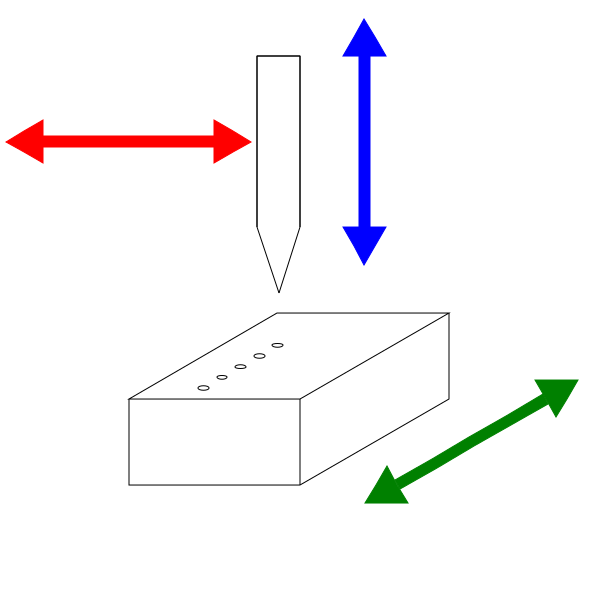
\includegraphics[width=4in]{figures/machines/xyzprobe.png}
	\caption[xyzprobe]
	{A probe move over a sample in either the x or z direction, and the sample moves along the y axis.  Repeated poking of the sample prints dots a simple but very versatile tool.}
\end{figure}


\begin{figure}
	\centering
	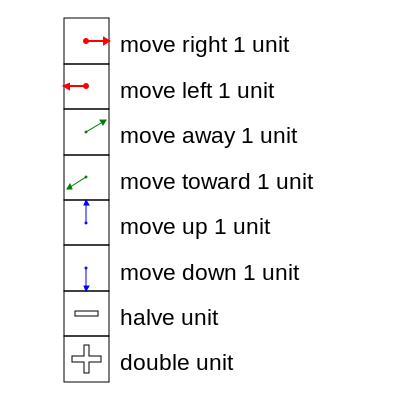
\includegraphics[width=4in]{figures/machines/basicmovements.png}
	\caption[basicmovements]
	{Basic geometric actions of machine control for an arbitrary machine that moves along three perpendicular axes.}
\end{figure}



\begin{figure}
	\centering
	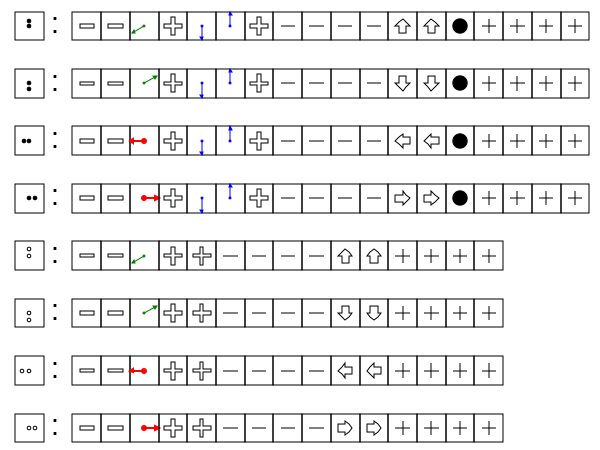
\includegraphics[width=4in]{figures/machines/actions05xx.png}
	\caption[actions05xx]
	{Dot actions from which symbols are constructed.}
\end{figure}


\subsection{2 and a half d printing and the Trash Robot icon token printer}


\begin{figure}
	\centering
	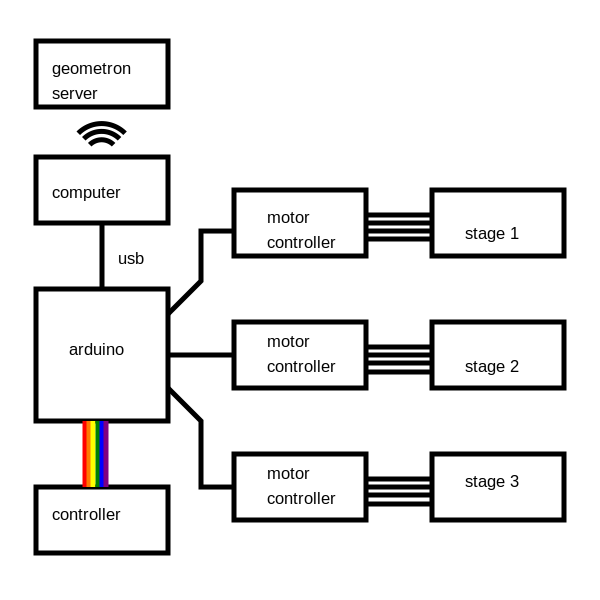
\includegraphics[width=4in]{figures/machines/printerblockdiagram.png}
	\caption[printerblockdiagram]
	{Block diagram of Trash Robot printer.  The motion stages are salvaged from DVD or CD ROM drives.  The motor drivers are off the shelf from Pololu Robotics.  The Arduino is the Arduino UNO, and the whole system including the motors gets power from the USB connected to a computer.  The computer can be used to interact with a Geoemtron server over the local network or on the global Internet to create programs which are copy/pasted into the Arduino IDE as described in the Trash Robot chapter.}
\end{figure}


\subsection{The wall robot}


\begin{figure}
	\centering
	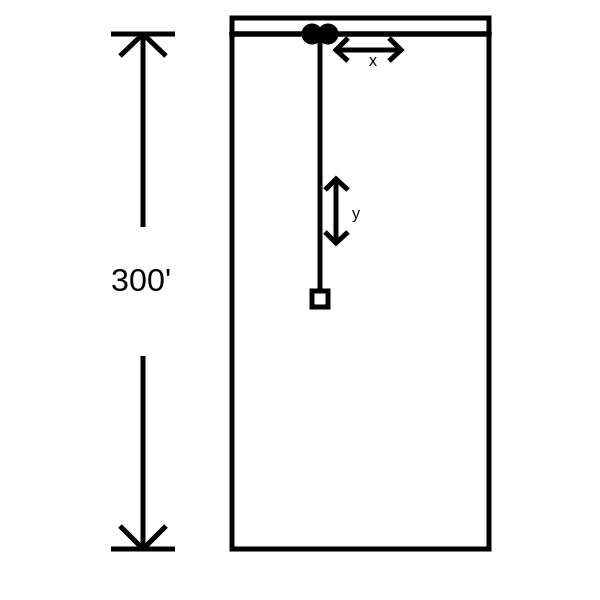
\includegraphics[width=4in]{figures/machines/buildingwallrobot.png}
	\caption[buildingwallrobot]
	{A hoist run along a rail going across the edge of a roof of a building can make a simple robot which can move to anywhere along the wall.}
\end{figure}


\subsection{Microfabrication and Nanofabrication}

\begin{figure}
	\centering
	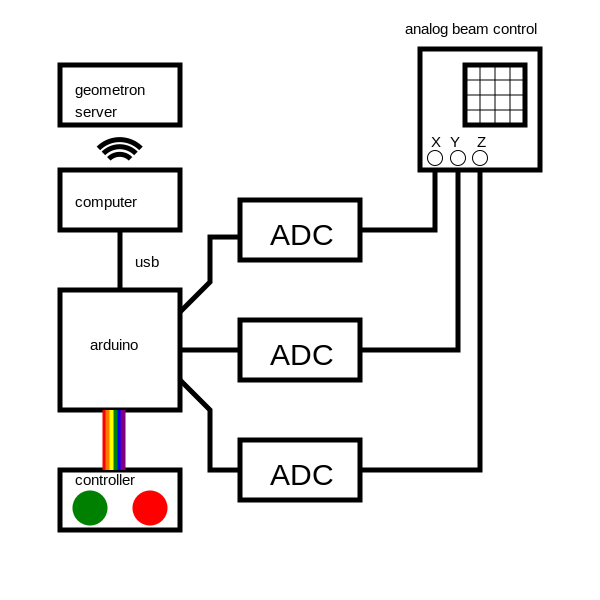
\includegraphics[width=4in]{figures/machines/eblblockdiagram.png}
	\caption[eblblockdiagram]
	{Block diagram of electron beam lithography Geometron robot.  The Arduino here drives three analog to digital converters.  Again the user can design a program for the beam path in a web browser using any computer, which can then also control and power the Arduino and its accessories.  In this case the controller only needs one huge green go button and one huge red stop button.}
\end{figure}

While we can use Geometron and Trash Robot control of electron beam lithography for all sorts of technology, as with the rest of the system our initial goal is simply to be able to print symbols and make self-replicating media.  One simple way to do that is to just program a ``write pixel'' action which is un-blanking the beam for a fixed amount of time, putting that in the pixel-write actions in the Hypercube at 0500 through 0503, along with xy control and printing identical symbols of pixels to the rest of the Trash Robot system.  To make this self-replicating we want to not just print a symbol on a substrate, but to make stamps which can be used to \emph{replicate} symbols from prints from the lithography system.  Ideally, as with the clay tokens documented in the last chapter of this work, an initial print can be used to make many stamps which in turn are used to make many of the final print.  While a fully demonstration of this technology is beyond the scope of the present manuscript, I believe this can be done relatively easily using spot size of about 1 micron, etching in polished brass wafers, using a negative resist.  Blasting the resist with extremely high doses of beam should be sufficient to reverse the effect of standard PMMA from a positive to a negative resist, making an etch process possible with just a single coat of thick PMMA spun on polished brass.  